\subsection{Framework}\label{section: zk-zkvm-framework}

Our high-level description of our framework as shown in the figure\ref{fig:zk-zkvm-framework} below:
\begin{figure}[!ht]
    \centering
    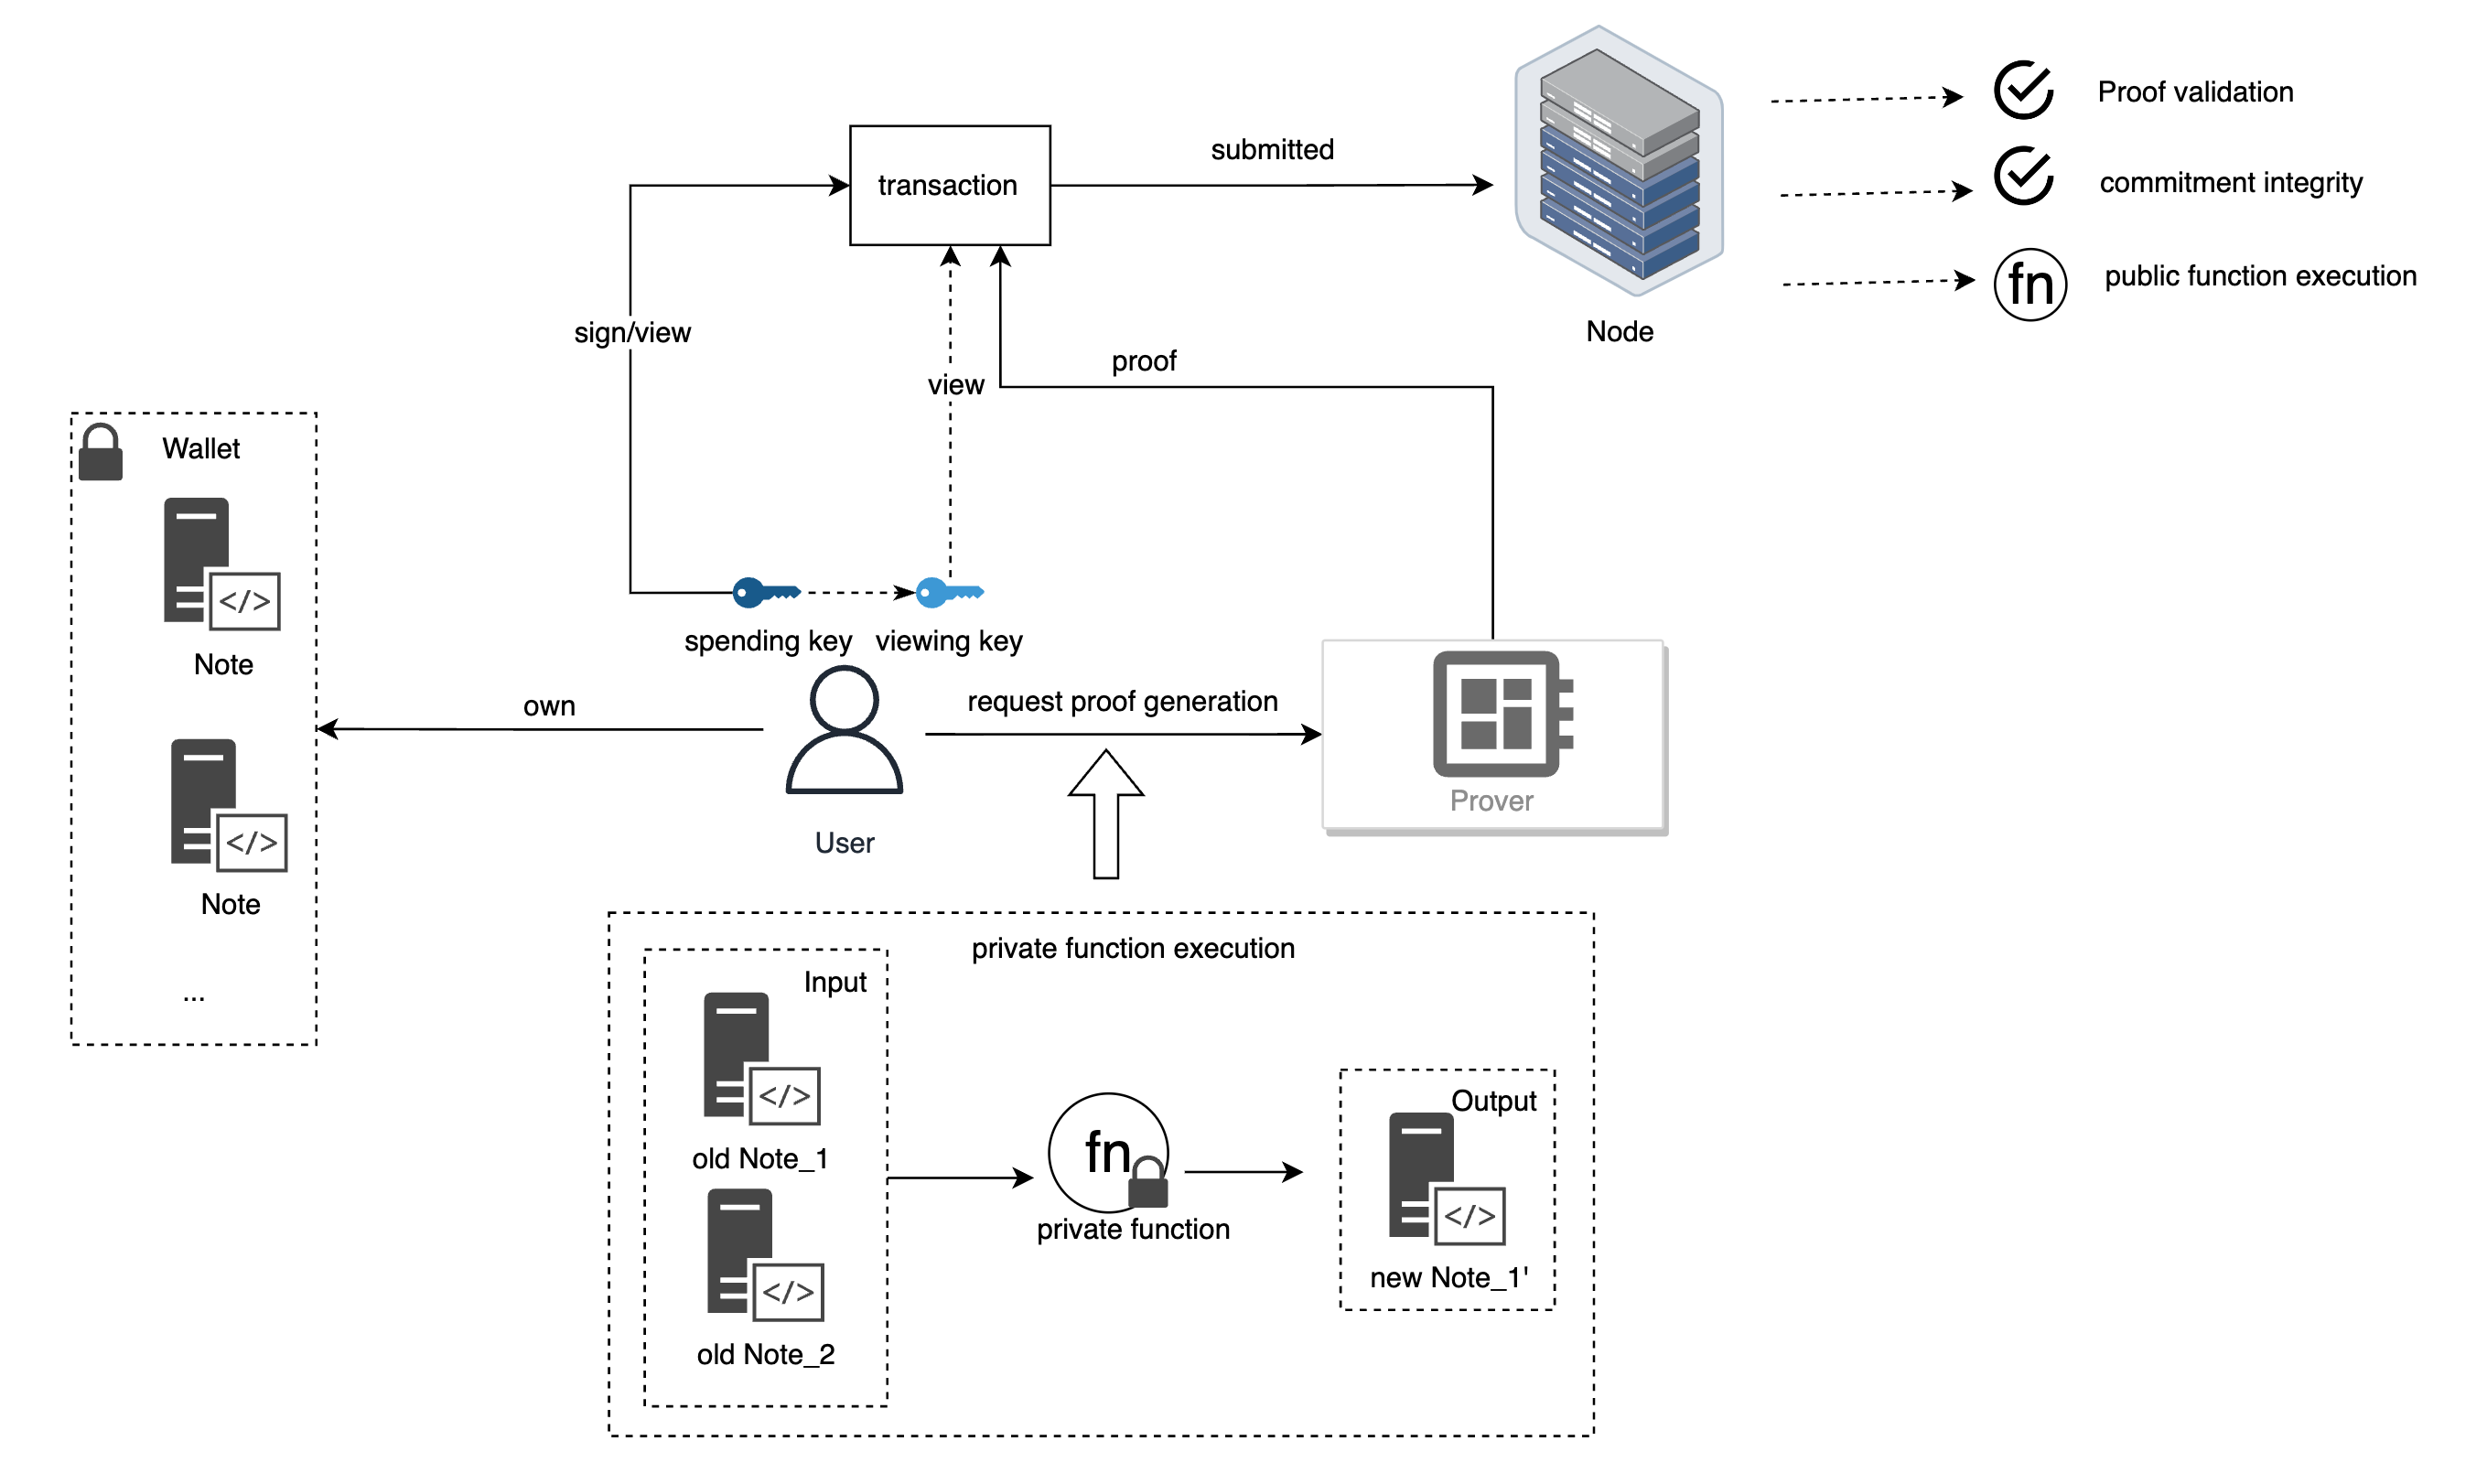
\includegraphics[width=0.6\textwidth]{zkzkvm framework.jpg}
    \caption{ZK-ZKVM Framework}
    \label{fig:zk-zkvm-framework}
\end{figure}

And the building blocks of our ZK-ZKVM are:

\textbf{Key System.}
\begin{itemize}
    \item The system will use a private key pair $(sk, vk)$ to enable spending and viewing of funds.
    \item The spending key $sk$ will be used to \textbf{sign} transactions such as transfer funds.
    \item The viewing key $vk$ will allow the holder to view transactions without being able to spend the funds nor change the state of owner.
    \item The system will ensure that transactions can only be signed using the correct spending key $sk$.
\end{itemize}
\bigskip

\textbf{Note Model.}
\begin{itemize}
    \item The system will use a UTXO (Unspent Transaction Output) model to track the ownership of state/funds.
    \item Each private transaction will create one or more new Notes, which can be spent in future transactions.
    \item The system will ensure that transactions can only spend Notes that are owned by the signer of the transaction.
    \item The Note reveals nothing but a meaningless string to other users.
\end{itemize}
\bigskip

\textbf{Private/Public execution.}
\begin{itemize}
    \item There are two kinds of functions for users in our system: private or public functions.
    \item Private functions have return values (also known as notes), while public functions do not.
    \item Private functions will be executed and proved by the signer of the transaction, using Key System and Notes as core techniques described above.
    \item Private state can be decrypted by the owner's key, while it can only be spent by the spending key and is read-only when decrypted by the viewing key.
    \item Public functions have a callback hook, which is used in the Node's execution and verification phase.
    \item Private functions can call Public functions, but not the other way around.
\end{itemize}
\bigskip

\textbf{Smart Contract.} As we said in earlier Chapter \ref{sec:zk-zkvm}, this is a ZK-ZKVM, which means it supports arbitrary smart contracts.